\selectlanguage{british}%

\chapter{Prologue}


\section{Overview}

A course in Quantum Mechanics (QM) typically leaves the reader with
a fuzzy view of the world. The founders of the subject, were able
to abstract out the mathematics from it's implications and interpretation.
The view that the wavefunction is the most complete description of
a system, known as the `Orthodox Copenhagen Interpretation', is among
the most popular. Einstein and Bohm, both played an important role
in challenging this belief. \\
Einstein showed \cite{EinsteinEPR} that if one makes reasonable assumptions
about nature (in the spirit of his relativity theories), then QM must
be incomplete. By incompleteness, he meant that the results of certain
experiments should be predictable precisely, but QM fails at doing
this. Thus he concluded that, QM must be treated as an intermediate
theory and that a more complete description of nature should be sought.
We will come back to this discussion. \\
Bohm challenged this view by realizing that one can't experimentally
refute the interpretation. His argument was that if for instance,
the predictions of QM fail to match with experiments, then one can
always add appropriate terms in the Hamiltonian until the difficulty
is resolved. He was already anticipating the modern form of particle
physics. To accurately account for interactions between particles,
one can postulate new force mediating particles, which was also done
in the history of the subject. However, one can't refute the interpretation
on grounds of inaccuracy in predictions. He therefore, aimed at, and
succeeded at constructing a complete quantum theory \cite{Bohm1},
now known as Bohmian Mechanics (BM)\footnote{Historically, Louis de Broglie had proposed a similar construction,
but abandoned the idea soon after. Bohm established it to be a consistent
theory.}. Its existence showed that we are not justified at believing the
interpretation, simply because there exists at least one alternative.

Returning to Einstein, %
\begin{comment}
as will be described in more detail
\end{comment}
Bell was able to construct a physical situation, that would test the
very requirements Einstein imposed on a complete quantum theory; he
was able to show that according to predictions of QM, \emph{such}
a complete description is impossible. This was verified experimentally
\cite{BellExp72,BellExpAspect81} (and was confirmed to be true, without
any possible loop-holes \cite{BellExpHensen2015}, only in 2015).\\
It might appear that Bell's test shows that QM is inconsistent with
BM. Upon looking at the details however, one can be convinced, that
this is not the case. Infact, Bell was among the first few to popularize
BM \cite{BellSpeakable}.

The discussion so far, is well known in the literature. However, certain
developments which followed the said work of Bohm, again lead to apparent
inconsistencies between BM and QM. These had not been satisfactorily
addressed in the literature and have become the subject of this thesis.
\\
For the sake of completeness, we merely name these. One must look
at the details, to be able to appreciate them. Greenberger, Horne
and Zeilinger (GHZ), constructed a test \cite{GHZ} that apparently
showed determinism can't exist, i.e. the notion that observables have
pre-defined values is inconsistent with QM. Developments due to Gleason
\cite{Gleason}, Bell himself \cite{BellOnHiddenVariables}, Kochen,
Specker \cite{KochenSpecker}, Peres and Mermin \cite{Peres,Mermin},
showed that the value an operator takes, must depend on the context
in which it is measured; context here refers to the complete set of
compatible operators.\\
The apparent contradiction must now be clear; BM is deterministic
and it is at odds with the notion of contextuality as well. 

\begin{comment}
\nomenclature{E}{Energy}\nomenclature{$m_0$}{intrinsic rest mass}\nomenclature{c}{speed of light}\nomenclature{p}{momentum}
\end{comment}



\section{The EPR argument}

%\begin{multicols}{3}

The EPR argument requires an entangled state, over two particles,
which was originally written as 
\[
\psi(q_{1},q_{2})=\int e^{-i(q_{1}-q_{2}+q_{0})p/\hbar}dp=\delta(q_{1}-q_{2}+q_{0}).
\]
In the modern notation, one can write this as 
\begin{eqnarray*}
\left|\psi\right\rangle  & = & \int\delta(q_{1}-q_{2}+q_{0})dq_{1}dq_{2}\left|q_{1}\right\rangle _{A}\left|q_{2}\right\rangle _{B}\\
 & = & \int\left|q\right\rangle _{A}\left|q+q_{0}\right\rangle _{B}dq.
\end{eqnarray*}
Similarly, one can write the same state as 
\begin{eqnarray*}
\left|\psi\right\rangle  & = & \int e^{-i(q_{1}-q_{2})p/\hbar}dpdq_{1}dq_{2}\left|q_{1}\right\rangle _{A}\left|q_{2}\right\rangle _{B}\\
 & = & \int e^{-iq_{1}p/\hbar}\left|q_{1}\right\rangle _{A}dq_{1}e^{iq_{2}p/\hbar}\left|q_{2}\right\rangle _{B}dq_{2}dp\\
 & = & \int\left|p\right\rangle _{A}\left|-p\right\rangle _{B}dp.
\end{eqnarray*}
where $A$ and $B$ label the particles. An attempt to reproduce the
precise argument, will not be made. Instead, we satisfy ourselves
with the following simplified argument. We assume the principle of
locality holds, which is to say that if two particles are sufficiently
far away, then any change made to one particle, should not influence
the other instantaneously. Given this assumption, consider two particles,
which are sufficiently far away and that their state is given by $\left|\psi\right\rangle $.
Now if the momentum of particle $B$ is measured by observer $B$,
then observer $B$, according to QM, will be able to predict the momentum
of particle $A$. Similarly, if the position of particle $B$ is measured,
then observer $B$ can predict the position of particle $A$. Further,
note that the choice made by observer $B$, can't influence particle
$A$, by the assumption of locality. It therefore follows that particle
$A$ had both it's position and momentum well defined, without being
measured. QM fails to yield the answer with precision, whereas as
we have shown, the answer was precise. Thus, we are forced to conclude
that QM is not a complete description of nature.

Einstein ended his paper with this remark: ``While we have thus shown
that the wave function does not provide a complete description of
the physical reality, we left open the question of whether or not
such a description exists. We believe, however, that such a theory
is possible.'' \cite{EinsteinEPR}


\section{Bell's Theorem\label{sec:Bell's-Theorem}}

Bell's work addresses and satisfactorily answers Einstein's open question,
of whether a \emph{such} a description exists. Consider the following
scenario. There are two observers, A and B, each has a particle. Each
observer, can measure two properties, call them $\hat{a}_{1},\hat{a}_{2}$
for observer A and $\hat{b}_{1},\hat{b}_{2}$ for observer B, which
yield a $\pm1$ outcome. Let $\left\langle \hat{a}_{i}\hat{b}_{j}\right\rangle $
represent the average value obtained by measuring the property $\hat{a}_{i}$
and $\hat{b}_{j}$ on the first and second particle respectively.
Consider the average given by $\left\langle \hat{B}\right\rangle =\left\langle \hat{a}_{1}\hat{b}_{1}\right\rangle +\left\langle \hat{a}_{1}\hat{b}_{2}\right\rangle +\left\langle \hat{a}_{2}\hat{b}_{1}\right\rangle -\left\langle \hat{a}_{2}\hat{b}_{2}\right\rangle $.
If one assumes local realism\footnote{Infact, an argument similar to EPR can be used to show that locality
entails realism.}, that is that the values $a_{i}$ takes are unaffected by those taken
by $b_{i}$ and that $\hat{a}_{i},\hat{b}_{j}$ have pre-defined values
(respectively), then $\left\langle \hat{B}\right\rangle \le2$. One
can check this quickly by a brute force substitution of $\pm1$ values,
in place of $a_{i},b_{j}$.

Consider now, the state $\left|\psi\right\rangle =\left(\left|+-\right\rangle -\left|-+\right\rangle \right)/\sqrt{2}$,
where $\hat{\sigma}_{x}\left|\pm\right\rangle =\pm\left|\pm\right\rangle $,
and $\hat{\sigma}_{x,y,z}$ are the Pauli matrices, given in the z-basis
as 
\[
\hat{\sigma}_{x}\doteq\left[\begin{array}{cc}
0 & 1\\
1 & 0
\end{array}\right],\,\hat{\sigma}_{y}\doteq\left[\begin{array}{cc}
0 & -i\\
i & 0
\end{array}\right],\,\hat{\sigma}_{z}\doteq\left[\begin{array}{cc}
1 & 0\\
0 & -1
\end{array}\right].
\]
Let $\hat{a}_{1}=\hat{\sigma}_{z}$ and $\hat{a}_{2}=\hat{\sigma}_{x}$,
while $\hat{b}_{1}=-\frac{\hat{\sigma}_{z}+\hat{\sigma}_{x}}{\sqrt{2}}$
and $\hat{b}_{2}=\frac{\hat{\sigma}_{z}-\hat{\sigma}_{x}}{\sqrt{2}}$.
Upon evaluating $\left\langle \hat{B}\right\rangle $ using the rules
of QM, one obtains $\left\langle \hat{B}\right\rangle =2\sqrt{2}\nleq2$.
This entails that our assumption, that of local realism, must be incorrect,
which settles the question: A \emph{local} hidden variable description
can not exist. The word hidden is used to represent information about
the state of the system, that is not contained in the wavefunction.
It is instructive to emphasize that a non-local description, may still
be possible. It is also important to note that, despite this non-locality,
one can't use QM to send signals instantaneously (superluminal communication
is not possible). This is known as the no-signalling theorem and can
be proven by showing that marginals in QM, don't depend on the system
which is traced out \cite{NielsenChuang}.


\section{Bohm's Theory, Bohmian Mechanics (condensed introduction)\label{sec:Bohm's-Theory,-Bohmian}}

Bohm gave a precise \cite{Bohm1}, but non-local description of quantum
phenomena. Let us start with non-interacting particles. A particle
is associated with (1) a position, $q$ \& momentum, $p$, precisely
defined and (2) a wavefunction $\psi=Re^{iS/\hbar}$. The postulates
of the theory are: (a) Evolution of the wavefunction, is governed
by Schrodinger's equation: $i\hbar\partial\psi/\partial t=-(\hbar^{2}/2m)\nabla^{2}\psi+V\psi$.
(b) The particle is guided by the wavefunction: $\dot{q}=p/m$ where
$p=\nabla S=\hbar\text{Im}(\nabla\psi/\psi)$. (c) The initial distribution
of the particles is given by $\rho(x)=\left|\psi\right|^{2}$.

The astute reader would've noticed that $\nabla S$ is just the probability
current, which entails that if the initial distribution satisfies
$\left|\psi(t_{0})\right|^{2}$, then it will do so at all times $t$,
thereafter. Before generalizing this to multiple particles, let us
first see a quick consequence of this formulation. In the Orthodox
Copenhagen interpretation, the double slit experiment is a source
of mystery and the which slit question, that of confusion. In BM,
since trajectories are well defined, one observes (see \prettyref{fig:Experimentally-observed-average})
that the particle goes through precisely one slit and then later,
forms the interference pattern. 
\begin{figure}
\begin{centering}
\includegraphics[width=0.7\textwidth]{Chapter1/Figs/Raster/singlePhotonTrajectory}
\par\end{centering}

\caption{Experimentally observed average single-photon trajectories. ``In
the case of single-particle quantum mechanics, the trajectories measured
in this fashion reproduce those predicted in the Bohm\textendash de
Broglie interpretation of quantum mechanics'' \cite{Kocsis1170}\label{fig:Experimentally-observed-average}}


\selectlanguage{english}%
\selectlanguage{english}%
\end{figure}
The wavefunction goes through both slits, and interferes to create
the pattern. If one of the slits is blocked, then since the wavefunction
can't interfere, the pattern is lost as expected. We haven't spoken
about measuring the particle yet, but if one notes that to measure
the particle, the potential at one of the slits must be changed, then
it is immediate that the interference pattern will be effected, since
the wavefunction is affected by the potential at both slits, even
if the particle passes through only one. One finds that by using the
following multi-particle generalization, and an appropriate measuring
scheme, one can show more precisely how the process of measuring effectively
destroys the pattern, replacing the mystery with clarity.

For $N$ interacting particles, we have $p_{i}=\nabla_{i}S(q_{1},q_{2},\dots,q_{N})$
where note that the momentum of the $i^{th}$ particle, depends on
the instantaneous positions of all the particles. Consequently, BM
is an explicitly non-local, but complete description. 

As a final remark, it must be added that spins can also be included
in BM, however, a particle is not associated with a specific spin,
only it's wavefunction is. For a spinor, say $\psi\equiv(\psi_{+},\psi_{-})^{T}$,
the generalization is that $p=\hbar\text{Im}((\psi,\nabla\psi)/(\psi,\psi))$
where $(.,.)$ represents inner product in the spin space $\mathbb{C}^{2}$.
A quick illustration is in order. Consider the following Stern-Gerlach
setup; Quantum effects are considered only along the $x$-axis. A
particle moves along the $z$-axis, with speed $v_{z}$, and it's
initial wavefunction, given by a Gaussian centred at the origin, say
$\psi(q_{x})=(1/\sqrt{2\pi}\sigma)e^{-q_{x}^{2}/2\sigma^{2}}$, viz.
$\left|\psi\right\rangle =\int dq\psi(q)\left|q\right\rangle $. It's
spin state is given by $\left|\chi\right\rangle =\left(\left|+\right\rangle +\left|-\right\rangle \right)/\sqrt{2}$,
where $\left|+\right\rangle $ and $\left|-\right\rangle $ are s.t.
$\sigma_{x}\left|\pm\right\rangle =\pm\left|\pm\right\rangle $. Along
the $z$-axis, a strong heterogeneous magnetic field is present, whose
action maybe captured by $H_{\text{int}}=a\hat{p}_{x}\otimes\hat{\sigma}_{x}$
where $a$ is a constant that quantifies the strength of the field.
Why this particular form works, will become clear momentarily. Assuming
that $a$ is large enough to neglect effects of free-evolution, we
have $\hat{U}(t)=e^{-ia\hat{p}_{x}\otimes\hat{\sigma}_{x}t/\hbar}$.
Thus, if the initial state is $\left|\Psi\right\rangle =\left|\psi\right\rangle \otimes\left|\chi\right\rangle $,
then 
\begin{eqnarray*}
\left|\Psi(t)\right\rangle  & = & \hat{U}(t)\left|\Psi\right\rangle \\
 & = & \frac{e^{-ia\hat{p}_{x}t/\hbar}\left|\psi\right\rangle \otimes\left|+\right\rangle +e^{ia\hat{p}_{x}t/\hbar}\left|\psi\right\rangle \otimes\left|-\right\rangle }{\sqrt{2}}\\
 & = & \frac{\left|\psi_{at}\right\rangle \otimes\left|+\right\rangle +\left|\psi_{-at}\right\rangle \otimes\left|-\right\rangle }{\sqrt{2}}
\end{eqnarray*}
where $\left|\psi_{q_{x0}}\right\rangle \equiv\int dq\psi(q_{x}-q_{x0})\left|q_{x}\right\rangle $,
viz. a Gaussian wavepacket centered at $q_{x0}$. One can plot $\left|\Psi\right|^{2}$,
as a function of $q_{z}$, using $q_{z}=v_{z}t$, schematically as
shown in the figure 
\begin{figure}
\begin{centering}
\includegraphics[width=0.8\textwidth]{Chapter1/Figs/Vectors/sg}
\par\end{centering}

\caption{Contour plot of $\left|\Psi(q_{x},t)\right|^{2}$ plotted for various
$t=q_{z}/v_{z}$, illustrating a Stern-Gerlach measurement. \label{fig:Contour-plot-of-Psi}}


\selectlanguage{english}%
\selectlanguage{english}%
\end{figure}
(see \prettyref{fig:Contour-plot-of-Psi}), where regions enclosing,
say $70\%$ of $\left|\Psi(q_{x})\right|^{2}$ have been outlined\footnote{Note that $\left|\Psi\right|^{2}=\left\langle \Psi|q_{x}\right\rangle \left\langle q_{x}|\Psi\right\rangle $,
where the spins are essentially traced over by the said expression}. So far, according to QM, if we measure the position of the particle,
then (given $\sigma\ll at$), obtaining the particle near $q_{x}=at$,
is as probable as finding it near $q_{x}=-at$. QM doesn't make a
deterministic prediction at this stage. According to BM, if in addition
to the wavefunction, we assume that the particle was initially at
some $q_{x}>0$, then we can predict precisely where the particle
will turn up. Infact, one can accomplish this with essentially no
calculation. Since $\dot{q}_{x}=\nabla S/m$, a single valued function,
it follows that trajectories of particles won't intersect, where recall
that $S$ is given by $\psi=Re^{iS/\hbar}$. Consequently, a particle
that starts with $q_{x}>0$, must follow the `up' trajectory, else
by symmetry, the trajectories will have to intersect. We conclude
therefore, that if $q_{x}>0$ initially, the particle has spin $\left|+\right\rangle $
and if $q_{x}<0,$ the spin must be $\left|-\right\rangle $. This
appears very clear and intuitive. A non-intuitive aspect of this,
is that we can't associate spins with particles, even though we can
predict precisely, the outcome of the experiment. This is manifested
by the observation that if $H_{\text{int}}\to-H_{\text{int}}$, which
practically amounts to reversing the heterogeneity of the magnet,
then $\sqrt{2}\left|\Psi(t)\right\rangle =\left|\psi_{-at}\right\rangle \otimes\left|+\right\rangle +\left|\psi_{at}\right\rangle \otimes\left|-\right\rangle $.
Again, if $q_{x}>0$ initially for a particle, it will follow the
`up' trajectory. However, now this corresponds to spin $\left|-\right\rangle $,
as opposed spin $\left|+\right\rangle $. We have thus demonstrated
that we can't associate spin uniquely to a particle, and that it must
only be associated with the wavefunction \cite{Detlef}. 

As an aside, it may be added that BM is known for removing the fundamental
role of an observer from the description of QM. This is accomplished,
roughly speaking, by introducing the positions of particles as well
defined, and then explaining the `collapse' of wavefunction, by means
of the particle's interaction with those in the environment, which
entails that the `collapsed wavefunction' serves as an effective wavefunction,
which can be used to describe the motion of the particle henceforth
\cite{Bohm2,Detlef}.


\section{Determinism: The GHZ test\label{sec:Determinism-The-GHZ}}

One drawback of Bell's test, was that it's statistical in nature.
The GHZ test \cite{GHZ}, takes this a step further and shows that
one can't even conceive of having pre-defined values. The construction
requires three observers with one particles each. Each observer can
measure two properties, $X$ and $Y$, with outcomes $\pm1$. We start
with the state $\sqrt{2}\left|\chi_{G}\right\rangle =\left|000\right\rangle -\left|111\right\rangle $
and note that for $\hat{A}:=\hat{\sigma}_{x}\otimes\hat{\sigma}_{y}\otimes\hat{\sigma}_{y}$,
$\hat{A}\left|\chi_{G}\right\rangle =\left|\chi_{G}\right\rangle $,
where the property $X$ is the projection of spin of the particle
along the $x$-axis and $Y$ is that along the $y$-axis. Thus a measurement
of $\hat{A}$ (the first observer measures $X$ and the other measure
$Y$), will yield $+1$ with certainty. Next, we define $\hat{B}:=\hat{\sigma}_{y}\otimes\hat{\sigma}_{x}\otimes\hat{\sigma}_{y}$
and $\hat{C}:=\hat{\sigma}_{y}\otimes\hat{\sigma}_{y}\otimes\hat{\sigma}_{z}$,
which by symmetry, must also yield $+1$ for the said state. If these
observables, $X$ and $Y$ had predefined values, then a measurement
of $\hat{A}\hat{B}\hat{C}$ would be equivalent to measuring $\hat{D}:=\hat{\sigma}_{x}\otimes\hat{\sigma}_{x}\otimes\hat{\sigma}_{x}$,
since $Y$s appear twice for each particle, and $Y^{2}=1$. Since
a measurement of each $\hat{A},$ $\hat{B}$ and $\hat{C}$ yields
a $+1$, it follows that a measurement of $\hat{D}$ therefore, must
also yield $+1$. However, $\hat{D}\left|\chi_{G}\right\rangle =-\left|\chi_{G}\right\rangle $,
which entails that a measurement of $\hat{D}$ must yield a $-1$.
Thus, we arrive at a contradiction and conclude that the assumption
that the properties $X$ and $Y$ had predefined values, must be incorrect.
One could object that $X$ and $Y$ are complementary properties (correspond
to non-commuting operators) and therefore it doesn't make sense to
assign values to these operators and treat them like numbers. This
objection is addressed by the contextuality tests.


\section{Contextuality: The Peres Mermin test\label{sec:Contextuality:-The-Peres}}

There've been various developments, of which the simplest, with effectively
the same consequence, is discussed: the Peres Mermin test \cite{Peres,Mermin}.
In this test also, we will show that pre-defined values can't exist,
but in addition, also define the notion of contextuality. Consider
the following set of operators 
\[
\hat{A}_{ij}\doteq\left[\begin{array}{ccc}
\hat{\mathbb{I}}\otimes\hat{\sigma}_{x} & \hat{\sigma}_{x}\otimes\hat{\mathbb{I}} & \hat{\sigma}_{x}\otimes\hat{\sigma}_{x}\\
\hat{\sigma}_{y}\otimes\hat{\mathbb{I}} & \hat{\mathbb{I}}\otimes\hat{\sigma}_{y} & \hat{\sigma}_{y}\otimes\hat{\sigma}_{y}\\
\hat{\sigma}_{y}\otimes\hat{\sigma}_{x} & \hat{\sigma}_{x}\otimes\hat{\sigma}_{y} & \hat{\sigma}_{z}\otimes\hat{\sigma}_{z}
\end{array}\right]
\]
which have the peculiar property that all operators along a row (and
along a column) commute. It is trivial to see that this holds for
the first two rows and the first two columns. To see that this holds
also for the last row and column, note the anti-commutation relation,
$\{\hat{\sigma}_{x},\hat{\sigma}_{y}\}=0$ and that $\sigma_{z}=i\sigma_{y}\sigma_{x}$,
which one may check explicitly. Another interesting property is that
the product of rows (columns) yield $\hat{R}_{i}=\mathbb{I}$ and
$\hat{C}_{j}=\mathbb{I}\,(j\neq3)$, $\hat{C}_{3}=-\mathbb{I}$, ($\forall\,i,j$)
where $\hat{R}_{i}\equiv\prod_{j}\hat{A}_{ij}$, $\hat{C}_{j}\equiv\prod_{i}\hat{A}_{ij}$.
This can be verified easily by using the aforesaid relations and the
fact that $\sigma^{2}=1$, for every Pauli matrix. Using this property
of $R_{i}$ and $C_{j}$, it is easy to show that no pre-defined values
for operators can exist. Let us assume that pre-defined values do
exist. Note that to get $C_{3}=-1$, we must have an odd number of
$-1$ assignments in the third column. In the remaining columns, the
number of $-1$ assignments must be even for each column. Thus, in
the entire square, the number of $-1$ assignments must be odd. Let
us use the same reasoning, but along the rows. Since each $R_{i}=1$,
we must have even number of $-1$ assignments along each row. Thus,
in the entire square, the number of $-1$ assignments must be even.
We have arrived at a contradiction and therefore we conclude that
our assumption that operators have predefined values, must be wrong.
One can infact construct the following inequality 
\[
\left\langle \hat{\chi}_{\text{PM}}\right\rangle =\left\langle \hat{R}_{1}\right\rangle +\left\langle \hat{R}_{2}\right\rangle +\left\langle \hat{R}_{3}\right\rangle +\left\langle \hat{C}_{1}\right\rangle +\left\langle \hat{C}_{2}\right\rangle -\left\langle \hat{C}_{3}\right\rangle \le4,
\]
if it is assumed that operators have predefined values. This can be
seen from an application of the aforesaid logic, which forbids an
assignment that yields only one column (row) as $-1$. The next best
assignment, viz. one that has two columns (or rows) set to $-1$,
yields $\left\langle \hat{\chi}_{\text{PM}}\right\rangle =4$ at best.
Ofcourse, according to QM $\left\langle \hat{\chi}_{\text{PM}}\right\rangle =6\nleq4$,
which is easier to verify experimentally. Thus a violation of the
Peres Mermin inequality, again entails that our assumption is wrong.
Note that unlike the GHZ test, the Peres Mermin test is (a) state
independent (no specific $\left|\chi\right\rangle $ is needed for
a violation) and (b) here, values of only commuting observables are
multiplied.

We are now in a position to discuss the notion of contextuality. We
begin with defining a non-contextual assignment to be one, where the
assignment depends only on the state ($\left|\chi\right\rangle $
+ hidden variables, if any) and the operator to which the assignment
is being made. It follows that we had tacitly assumed a non-contextual
assignment, that resulted in a contradiction. If we allow for the
value of an operator, to depend on the context in which it is measured,
where the context is meant to refer to a set of compatible observables,
then the contradiction won't arise. For instance, if we imagine that
all observables yield a $+1$, except $\hat{A}_{33}$ which yields
a $-1$ if measured with $\hat{A}_{32},\,\hat{A}_{31}$ and yields
a $+1$ if measured with $\hat{A}_{23},\,\hat{A}_{13}$. If this doesn't
appear entirely unsatisfactory, then you're on the right track and
are encouraged to read the more detailed description given in \prettyref{chap:An-Alternative-to-Contextuality}
(more specifically, Subsection \prettyref{sub:Contextual,-Memory-Model}).\selectlanguage{english}%

